\section{The ATLAS detector}
\label{sec:detector}

The ATLAS detector is a multi-purpose detector at the Large Hadron Collider (LHC). It is a nearly hermetic detector built to measure the trajectory and momenta of particles arising from proton-proton collisions. 

The Inner Detector (ID) measures the trajectory of charged particles immersed in a multi-tesla solenoidal magnetic field, thus providing precise momentum measurements. It is composed of three detector technologies: silicon pixels, silicon strips (SCT), and a transition radiation tracker (TRT). It is surrounded by non-compensating electromagnetic and hadronic calorimeters, whose active material are liquid argon and scintillator, respectively.

Outside the ID and calorimeters, the muon spectrometer (MS) exists to measure the trajectory of muons immersed in a multi-tesla toroidal magnetic field. The MS consists of three concentric shells, or ``layers'', split into barrel and endcap regions. Four detector technologies are used: monitored drift tubes (MDTs) and cathode strip chambers (CSCs) provide precise momentum measurements, and resistive plate chambers (RPCs) and thin gap chambers (TGCs) provide fast measurements for triggering at the 40 MHz LHC collision rate. The MDTs and the CSCs are the focus of this note.

The MDTs consist of $\sim\!400,000$ drift tubes and cover the most of the MS. They are used up to $|\eta| < 2.7$ in the middle and outer layers, and up to $|\eta| < 2.0$ in the inner layer, where the incident particle flux becomes unmanageable. The tubes are grouped into chambers which consist of three to eight layers of drift tubes. The gas mixture in the tubes is 93\% Ar and 7\% $\text{CO}_2$, which have a maximal drift time of about $\sim\!700$ ns.

The CSCs are deployed in the region $2.0 < |\eta| < 2.7$ of the endcap inner layer, which is the region closest to the beam pipe and subject to the largest incident particle flux. The CSCs are multiwire proportional chambers with cathode planes segmented into strips in orthogonal directions for measurements of $\eta$ and $\phi$. In this study, only the $\eta$ strips are considered in the measurement of hit rates because they are finer than the $\phi$ strips, and because they offer information about dependence of the hit rate on the distance from the beam pipe. Neighboring hit strips are clustered to reflect an incident particle, and the spatial coordinates are derived from a charge-dependent interpolation of this cluster.

Some naming conventions are adopted in this note. The MS is divided in the $\phi$-plane into 16 sectors, 8 of which are referred to as ``large'' (L) sectors and 8 of which are ``small'' (S), determined by their coverage in $\phi$. The three concentric layers are referred to as the Inner, Middle, and Outer layers according to the distance from the interaction point (IP). Within a layer, the chambers are further divided into $\eta$ stations between 1 and 8, also according to their distance from the IP. Last, the positive (negative) $z$ region of the MS is referred to as the A (C) side.

Groups of chambers are designated with acronyms of this information -- for example, the MDT EIL1 chambers refer to the large sectors of the first $\eta$ station of MDT chambers in the inner endcap, including all $\phi$ sectors. In this note, the hit rates are not divided into $\phi$ sectors since the hit rates are generally symmetric in this coordinate. These conventions are shown schematically in Figure~\ref{fig:detector-ms}.

\begin{figure}
  \begin{center}
    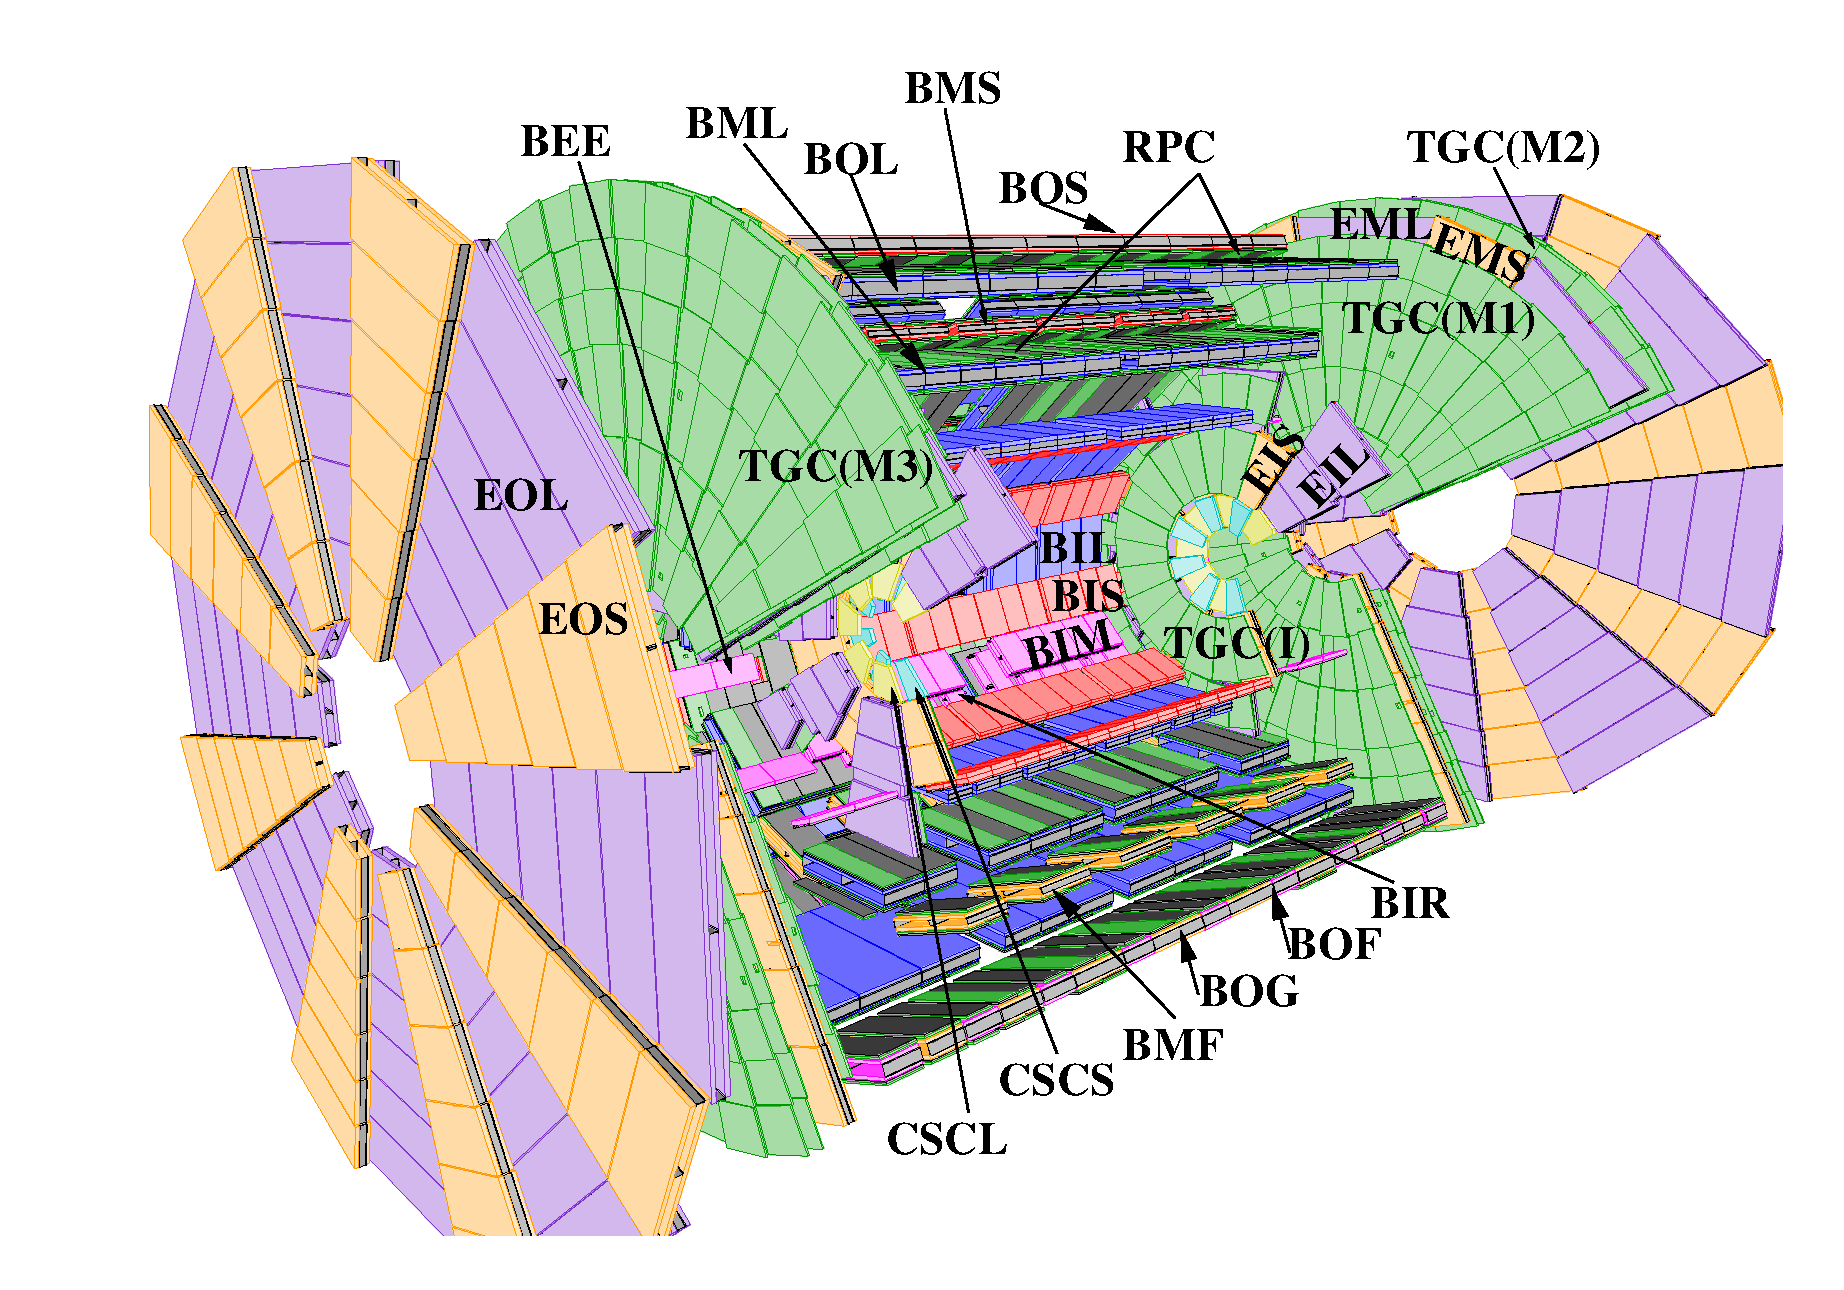
\includegraphics[width=0.80\textwidth]{./figures/TDR_Muon_system_Initial.pdf}
    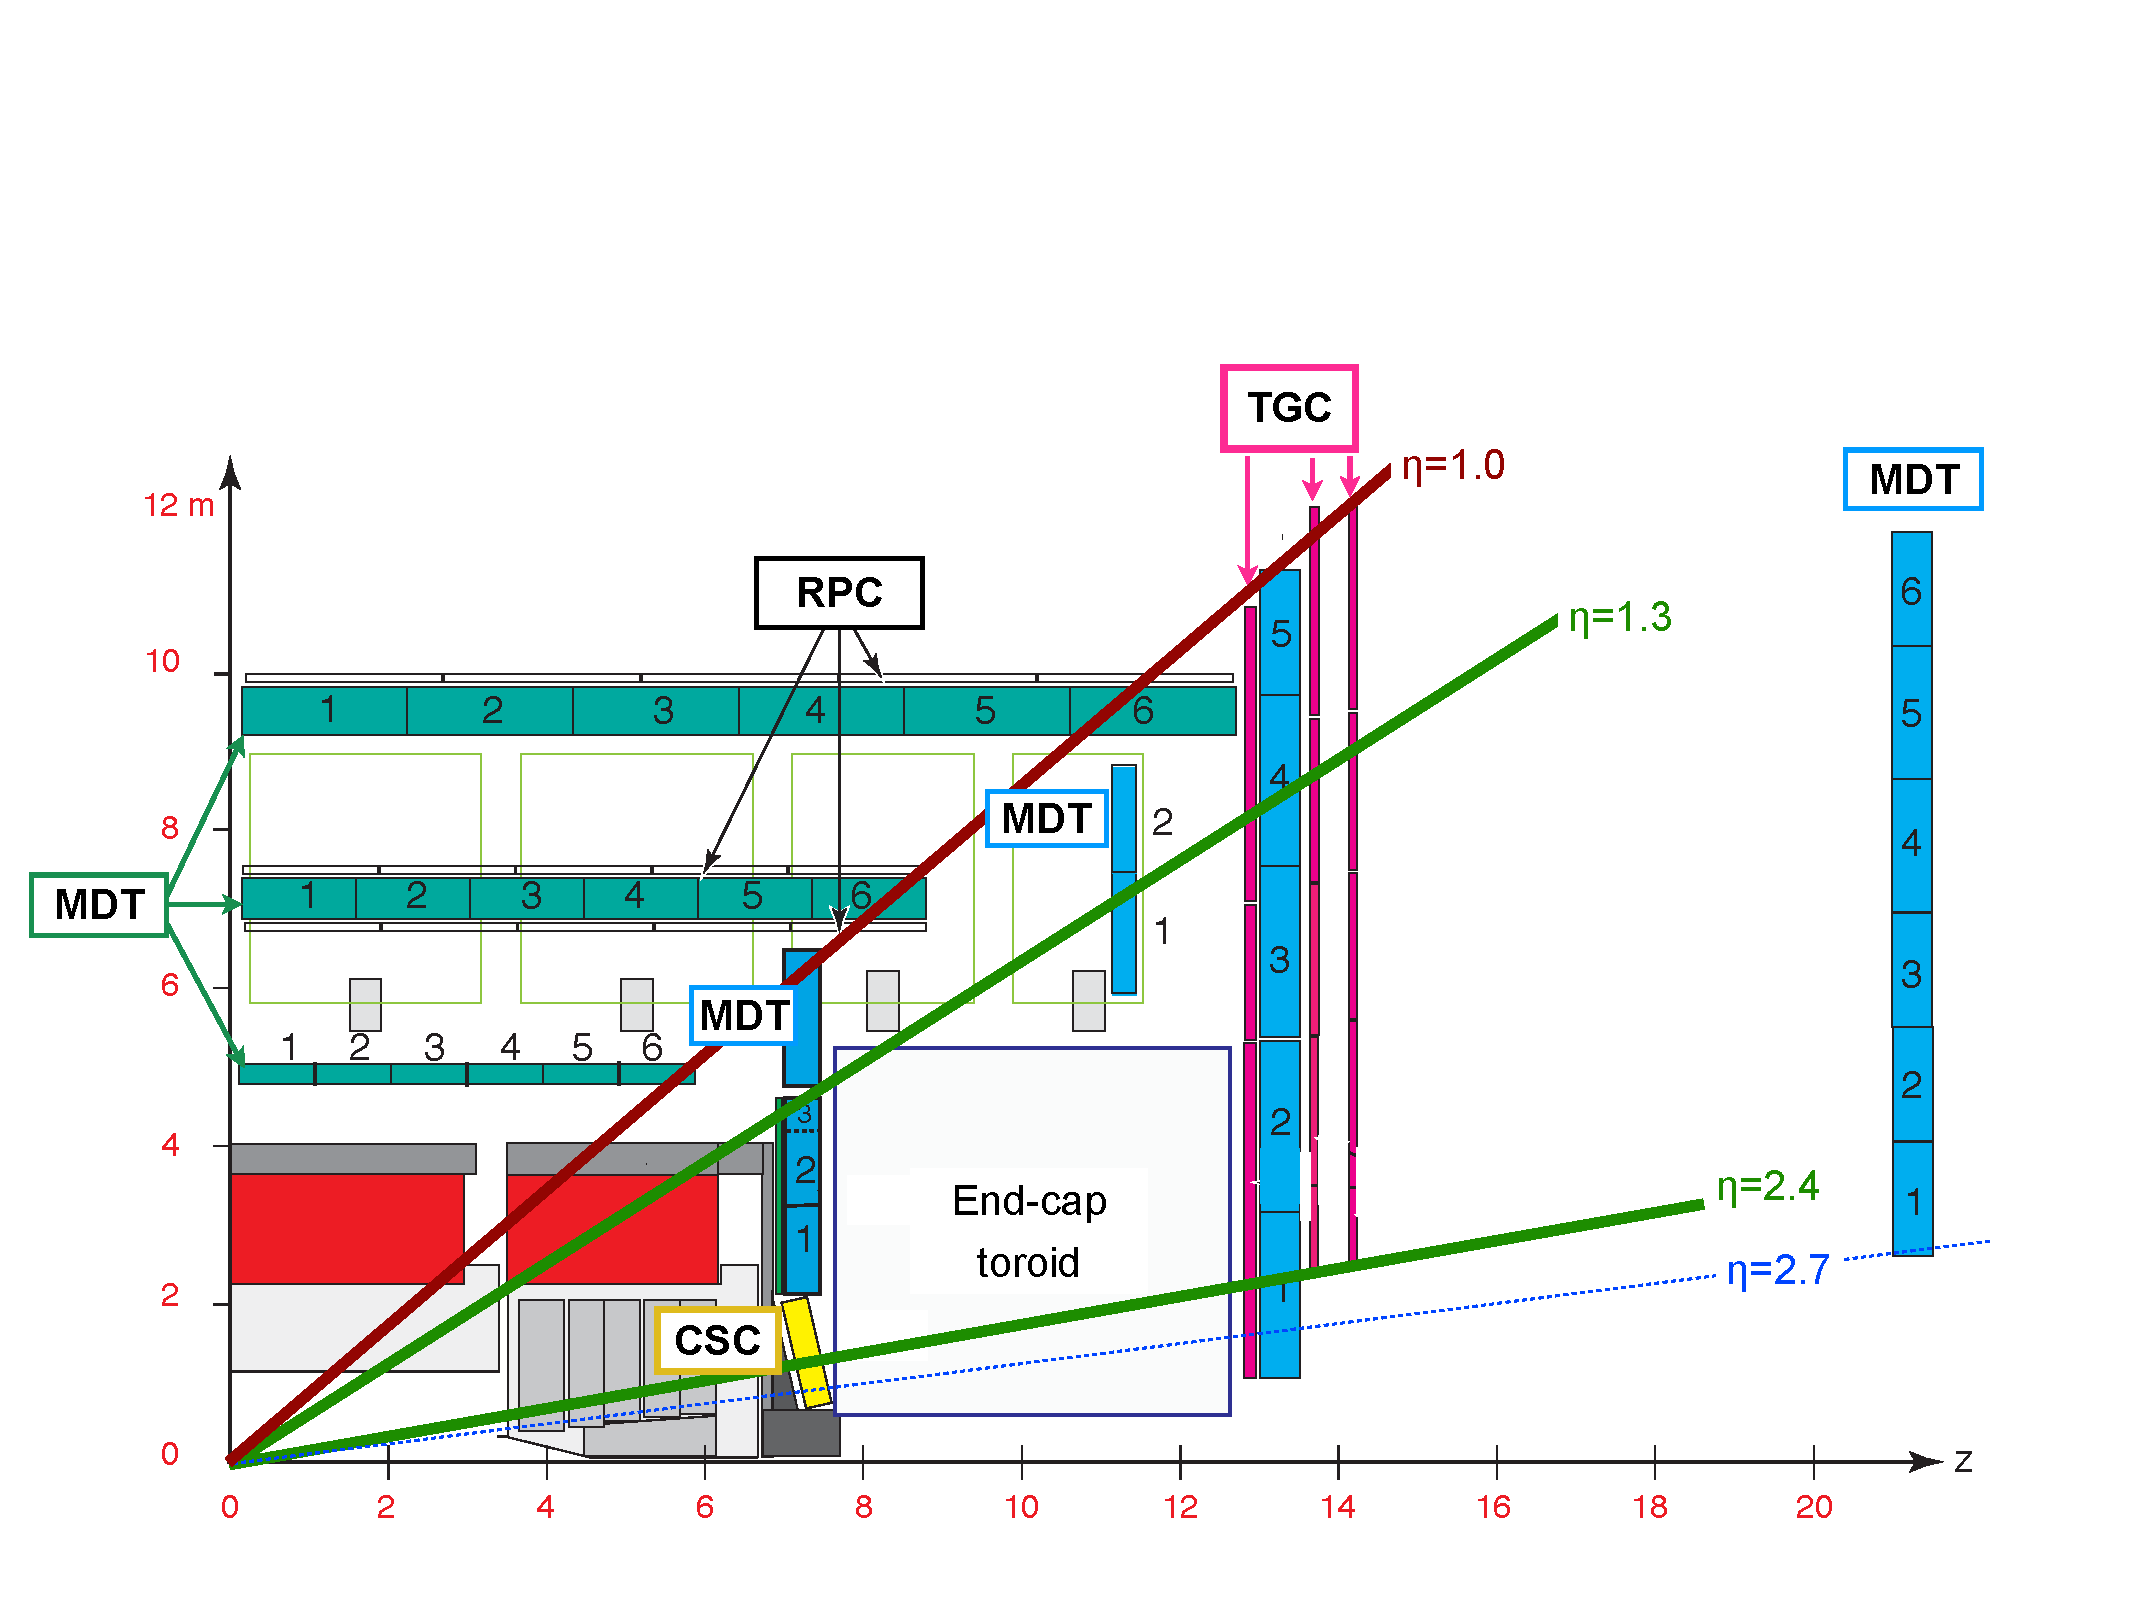
\includegraphics[width=0.80\textwidth]{./figures/TRIG-2012-03_fig_01.pdf}
    \caption{Schematic pictures \cite{PERF-2007-01} showing a cross-section (top) and quarter-section (bottom) of the muon system. The MDT chambers in the barrel are arranged in three concentric cylindrical shells around the beam axis. In the endcap region, muon chambers form large wheels, perpendicular to the z-axis. In the forward region, CSC is used in the innermost tracking layer. The RPC and TGC chambers are arranged in three layers (called stations) as indicated in the figure.}
    \label{fig:detector-ms}
  \end{center}
\end{figure}


